\chapter{Architectural Design}

\section{Overview}
The CKB platform system is composed by a 3-tier architecture.\\
Its software application architecture is organized into three logical tiers: the presentation tier, or user interface; the application tier, where data is processed; and the data tier, where the data associated with the application is stored and managed.

\begin{figure}[H]
\centering
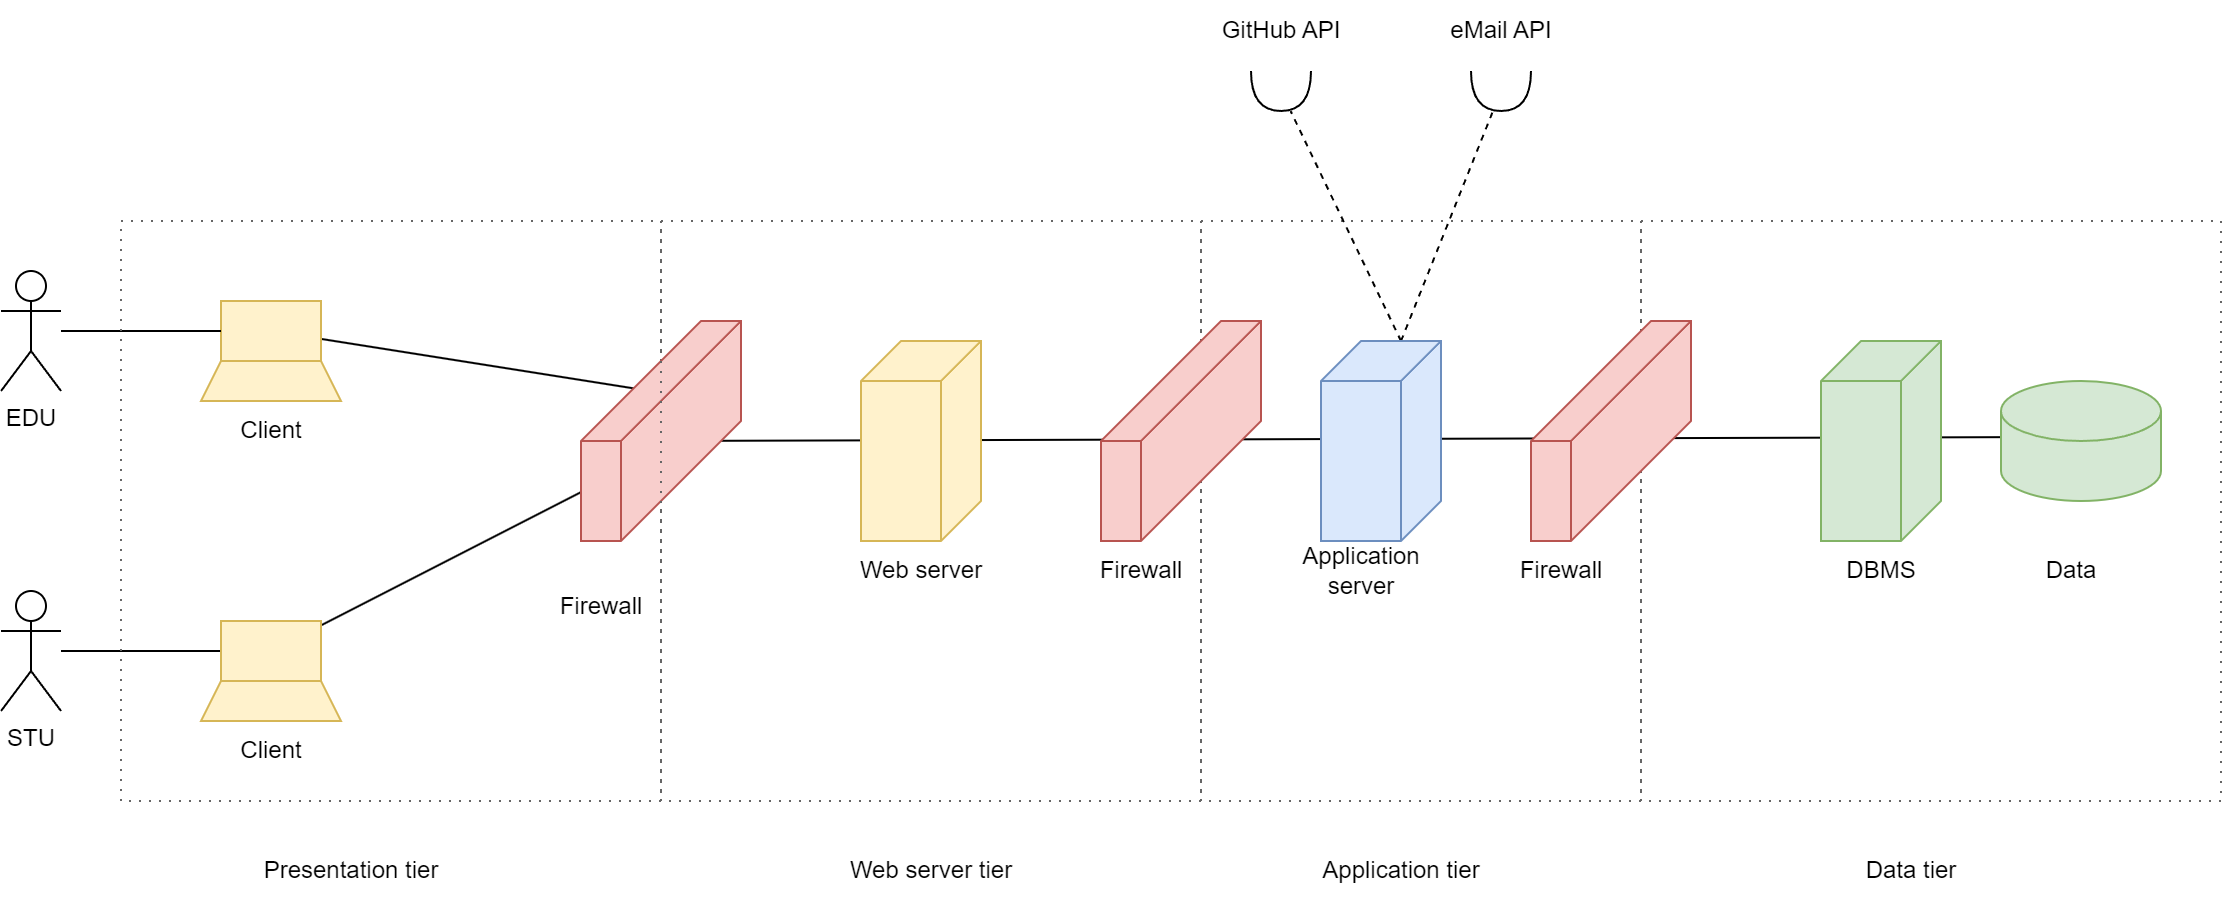
\includegraphics[width=0.8\textwidth]{images/diagrams/high_level_diagram.png}
\caption{High level components diagram}
\end{figure}

The service will be accessed through a web interface, employing a Single Page Application (SPA). Utilizing an SPA is ideal for this application, as it facilitates extensive interaction without necessitating frequent page reloads.\\
The system's architecture is structured into distinct layers, with application servers interacting with a database management system and utilizing APIs for data retrieval and storage. {\color{red}Adhering to REST standards, the application servers are intentionally designed to be stateless, -e le sessioni di log in come ce le gestiamo?-} while the system will include more than one firewall to ensure security.\\

\section{Component view}
The system is composed by the following components:

\begin{figure}[H]
\centering
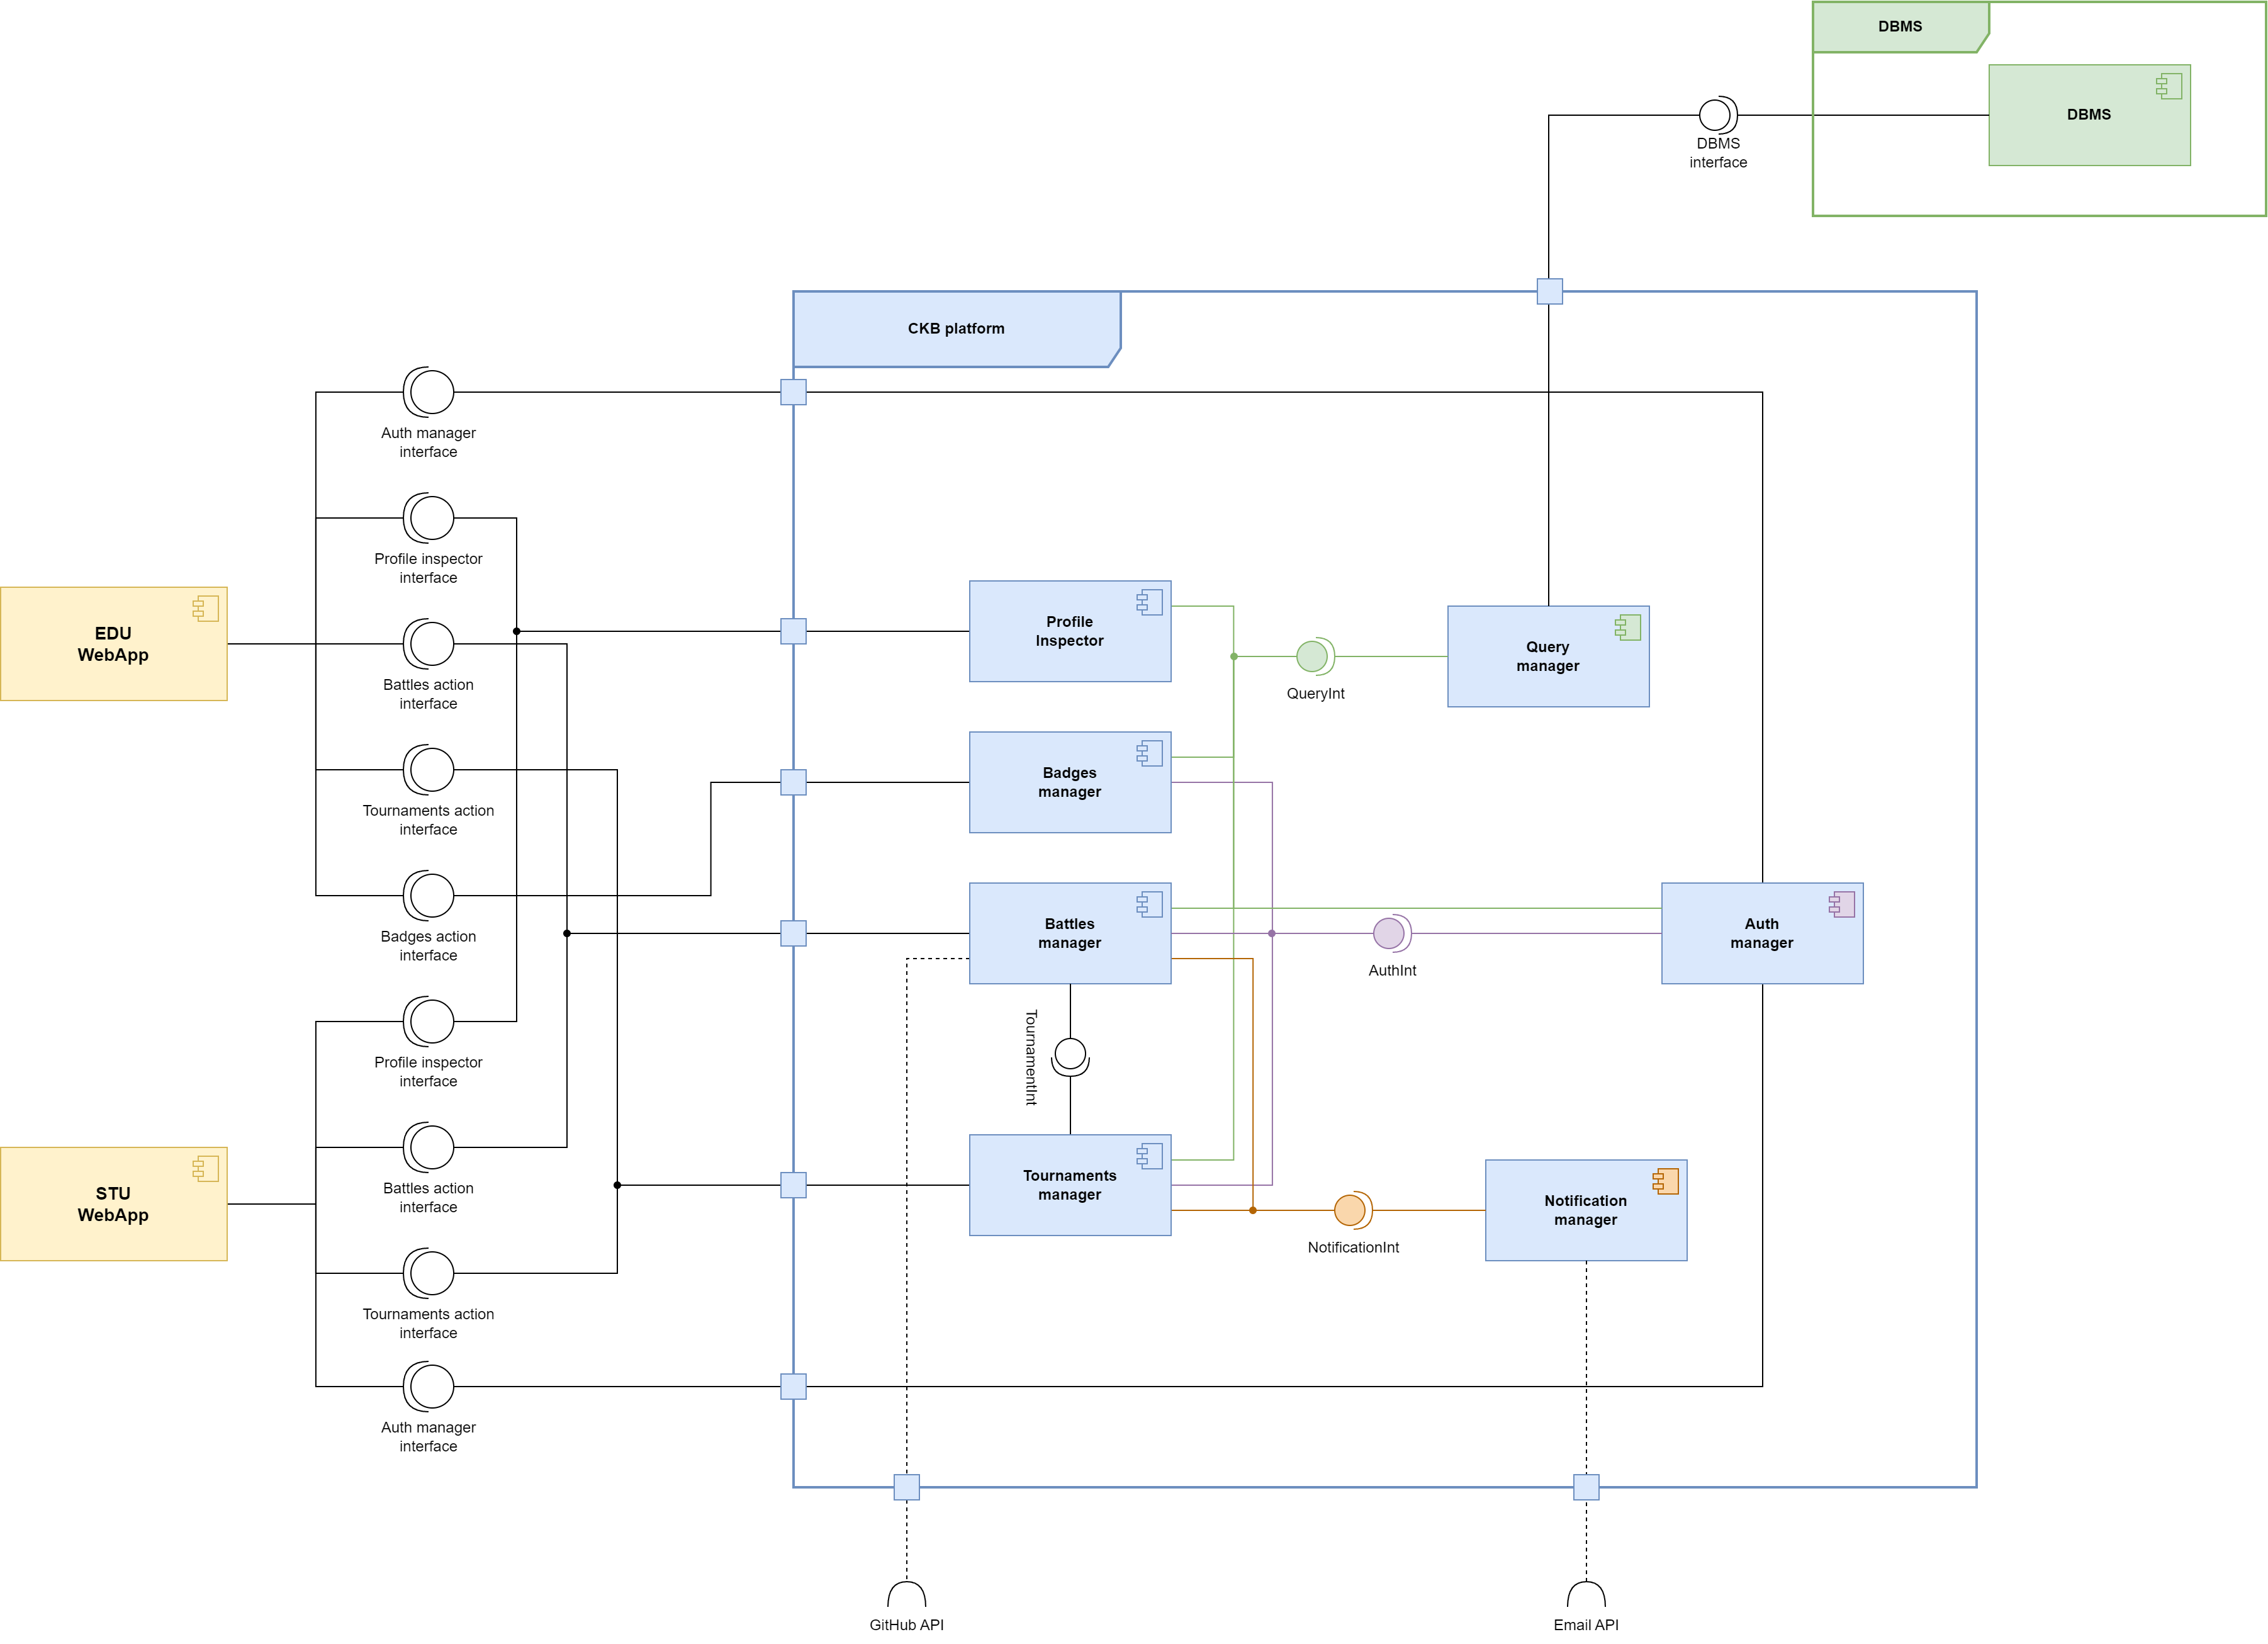
\includegraphics[width=0.8\textwidth]{images/diagrams/component_diagram.png}
\caption{Component diagram}
\end{figure}

{\color{red}Qui va bene aver raggruppato le interfacce oppure vanno messe singolarmente, una per ogni endpoint?}